%%%%%%%%%%%%%%%%%%%%%%%%%%%%%%%%%%%%%%%%%%%%%%%%%%%%%%%%%%
\begin{frame}
  \begin{center}
    {\Large Quick Overview of Python}
  \end{center}
\end{frame}

%%%%%%%%%%%%%%%%%%%%%%%%%%%%%%%%%%%%%%%%%%%%%%%%%%%%%%%%%%%%%%%%%%%%%%%%%%%%%%%%%%%
\begin{frame}[fragile]  \frametitle{Quiz}
Find Factorial of a Number
\begin{center}
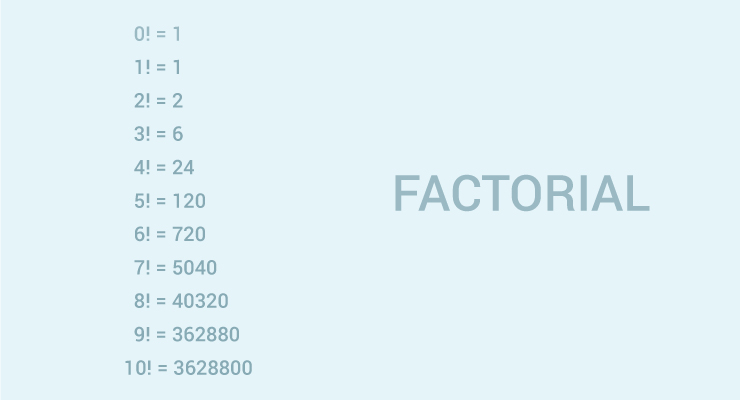
\includegraphics[width=\linewidth,keepaspectratio]{factorial}
\end{center}
\end{frame}



%%%%%%%%%%%%%%%%%%%%%%%%%%%%%%%%%%%%%%%%%%%%%%%%%%%%%%%%%%%%%%%%%%%%%%%%%%%%%%%%%%%
\begin{frame}[fragile]  \frametitle{Solution}
Without recursion
\begin{lstlisting}
def myfactorial(n):
	factorial = 1
	# check if the number is negative, positive or zero
	if num < 0:
		print("Sorry, factorial does not exist for negative numbers")
	elif num == 0:
		return 1
	else:
		for i in range(1,n + 1):
       			factorial = factorial*i
	return factorial

myfactorial(7)
\end{lstlisting}
\end{frame}

%%%%%%%%%%%%%%%%%%%%%%%%%%%%%%%%%%%%%%%%%%%%%%%%%%%%%%%%%%%%%%%%%%%%%%%%%%%%%%%%%%%
\begin{frame}[fragile]  \frametitle{Solution}
With recursion
\begin{lstlisting}
def recur_factorial(n):
   if n == 1:
       return n
   else:
       return n*recur_factorial(n-1)

recur_factorial(7)
\end{lstlisting}
\end{frame}

%%%%%%%%%%%%%%%%%%%%%%%%%%%%%%%%%%%%%%%%%%%%%%%%%%%%%%%%%%%%%%%%%%%%%%%%%%%%%%%%%%%
\begin{frame}[fragile]  \frametitle{What is Python?}
\begin{itemize}
\item Python is an interpreted, object-oriented, high-level programming language with dynamic semantics.
\item Python is open source, free and cross-platform.
\item Python provides high-level built in data structures.
\item Python is useful for rapid application development.
\item Python can be used as a scripting or glue language.
\item Python emphasizes readability.
\item Python supports modules and packages.
\end{itemize}
\end{frame}

%%%%%%%%%%%%%%%%%%%%%%%%%%%%%%%%%%%%%%%%%%%%%%%%%%%%%%%%%%%%%%%%%%%%%%%%%%%%%%%%%%%
\begin{frame}[fragile]  \frametitle{The Zen of Python}
{\em \large There should be one - and preferably only one - obvious way	to do it.}



Pythonic way of doing things.
\end{frame}

%%%%%%%%%%%%%%%%%%%%%%%%%%%%%%%%%%%%%%%%%%%%%%%%%%%%%%%%%%%%%%%%%%%%%%%%%%%%%%%%%%%
\begin{frame}[fragile]  \frametitle{The Python shell, I}
  \begin{itemize}
  \item Python can be run from ``shell'', IDE, Notebook
 \item Shell/Command Line:
\begin{lstlisting}
> python

Python 3.5.3 | packaged by conda-forge | (default, May 12 2017, 16:16:49) [MSC v.1900 64 bit (AMD64)] on win32
Type "help", "copyright", "credits" or "license" for more information.
>>>
\end{lstlisting}
\item Start writing commands/expressions at the $>>>$ prompt.
\end{itemize}
\end{frame}

%%%%%%%%%%%%%%%%%%%%%%%%%%%%%%%%%%%%%%%%%%%%%%%%%%%%%%%%%%%%%%%%%%%%%%%%%%%%%%%%%%%
\begin{frame}[fragile]\frametitle{The Python shell, II}
\begin{itemize}
\item Expressions are evaluated and the result is printed:
	\begin{lstlisting}
	>>> 2+2
	4
	\end{lstlisting}

\item Line continuation with \\ 
\begin{lstlisting}
>>> "hello" + \
... " world!"
'hello world!'
\end{lstlisting}
\item The prompt changes to `\texttt{...}' on continuation lines and for loops, function definitions, etc.
\end{itemize}
\end{frame}

%%%%%%%%%%%%%%%%%%%%%%%%%%%%%%%%%%%%%%%%%%%%%%%%%%%%%%%%%%%%%%%%%%%%%%%%%%%%%%%%%%%
\begin{frame}[fragile]  \frametitle{Overall Syntax}
\begin{itemize}
\item Comments are indicated with ``\#''
\item Multiple statements on the same line are separated with ``;''
\item No semicolon at the end of lines.
%\item a long line continue on next with ``\'' (it is not always needed)
\item Scope is obtained through indentation. 
\item Always indent next line if ``:'' is at the end of current line.
\item One script is can be run or imported by other modules.
%\item  assignment uses the equal sign ``=''
\end{itemize}
\end{frame}


%%%%%%%%%%%%%%%%%%%%%%%%%%%%%%%%%%%%%%%%%%%%%%%%%%%%%%%%%%%%%%%%%%%%%%%%%%%%%%%%%%%
\begin{frame}[fragile]  \frametitle{Assignment}
\begin{itemize}
\item Assignment creates references, not values:
\lstinline{tmp = "hello"; tmp = 10}
the first string will be deallocated
%\item Contrary to C, assignment do not have value:
%\lstinline{y = (x = x + 1)}
% is invalid
\item As in C programming: \lstinline{x += 1} is valid
\item Pre/post increment/decrements: \lstinline{x++; ++x; x--;--x} are invalid
\item Multiple assignment (references to a unique object):\lstinline{x=y=z=1}
\item Multiple assignments: \lstinline{(x,y,z)=(3.5,5.5,`string')}
\item  Example of swapping variables value: \lstinline{(x,y)=(y,x)}
\end{itemize}
\end{frame}

%%%%%%%%%%%%%%%%%%%%%%%%%%%%%%%%%%%%%%%%%%%%%%%%%%%%%%%%%%%%%%%%%%%%%%%%%%%%%%%%%%%%
%\begin{frame}[fragile]  \frametitle{Special variables}
%\begin{itemize}
%\item Python relies on many special variables that can be accessed by your code.
%\item One is the \lstinline{name} variables.
%\item When a module is run, it contains the string \lstinline{main}.
%\item When the module is imported, it contains the modules name.
%\item You can add code that runs only when a module is called directly:\lstinline{if __name__ == __ main__: test()}
%\end{itemize}
%\end{frame}

%%%%%%%%%%%%%%%%%%%%%%%%%%%%%%%%%%%%%%%%%%%%%%%%%%%%%%%%%%%%%%%%%%%%%%%%%%%%%%%%%%%
\begin{frame}[fragile]\frametitle{Built-in object types}
  \begin{itemize}
  \item Numbers : \lstinline{3.1415, 1234, 999L, 3+4j}
  \item Strings : \lstinline{`spam', ``guido's''}
  \item Lists : \lstinline{[1, [2, `three'], 4]}
   \item Dictionaries :\lstinline|{`food':`spam', `taste':`yum'}|
  \item Tuples : \lstinline{(1,`spam', 4, `U')}
  \item Sets: \lstinline|{1,2,3,'foo','bar'}|
%  \item Files : \lstinline{text = open(`eggs', `r').read()}
  \end{itemize}
\end{frame}

%%%%%%%%%%%%%%%%%%%%%%%%%%%%%%%%%%%%%%%%%%%%%%%%%%%%%%%%%%%%%%%%%%%%%%%%%%%%%%%%%%%
\begin{frame}[fragile]\frametitle{Numbers}
  \begin{itemize}
  \item Integers : \lstinline{1234, -24, 0}
  \item Unlimited precision integers : \lstinline{ 999999999999L}
  \item Float : \lstinline{3.1415, 2.7122}
   \item Oct and hex :\lstinline|0177, 0x9ff|
  \item Complex : \lstinline{3+4j, 3.0+4.0j, 3J}
  \end{itemize}
\end{frame}

%%%%%%%%%%%%%%%%%%%%%%%%%%%%%%%%%%%%%%%%%%%%%%%%%%%%%%%%%%%%%%%%%%%%%%%%%%%%%%%%%%%
\begin{frame}[fragile]\frametitle{Strings (immutable sequences)}
  \begin{itemize}
  \item single quote \lstinline{s1 = `egg'}
\item double quotes \lstinline{s2 = ``spam's''}
\item triple quotes \lstinline{block = ```...'''}
\item concatenate \lstinline{s1 + s2}
\item repeat \lstinline{s2 * 3}
\item index,slice \lstinline{s2[i], s2[i:j]}
\item length \lstinline{len(s2)}
\item formatting \lstinline|``a {} parrot''.format(`dead')|
\item iteration \lstinline{for x in s2 # x loop through each character of s2}
\item membership \lstinline{`m' in s2}
  \end{itemize}
\end{frame}

%%%%%%%%%%%%%%%%%%%%%%%%%%%%%%%%%%%%%%%%%%%%%%%%%%%%%%%%%%%%%%%%%%%%%%%%%%%%%%%%%%%
\begin{frame}[fragile]\frametitle{Lists}
  \begin{itemize}
  \item Ordered collections of arbitrary objects
  \item Accessed by offset
  \item Variable length, heterogeneous, arbitrarily nest-able
  \item Mutable sequence
  \item Arrays of object references
  \end{itemize}
\end{frame}

%%%%%%%%%%%%%%%%%%%%%%%%%%%%%%%%%%%%%%%%%%%%%%%%%%%%%%%%%%%%%%%%%%%%%%%%%%%%%%%%%%%
\begin{frame}[fragile]\frametitle{Lists operations}
  \begin{itemize}
  \item empty list \lstinline{L = []}
    \item create list \lstinline{L1 = range(4)}
  \item four items \lstinline{L2 = [0, 1, 2, 3]}
  \item nested \lstinline{L3 = ['abc', ['def', 'ghi']]}
  \item index \lstinline{L2[i], L3[i][j]}
  \item slice  \lstinline{L2[i:j]}, length \lstinline{len(L2)}
  \item concatenate \lstinline{L1 + L2}, repeat \lstinline{L2 * 3}
  \item iteration \lstinline{for x in L2}, membership \lstinline{3 in L2}
  \item methods \lstinline{L2.append(4), L2.sort(), L2.index(1), L2.reverse()}
  \item shrinking \lstinline{del L2[k], L2[i:j] = []}
  \item assignment \lstinline{L2[i] = 1, L2[i:j] = [4,5,6]}

  \end{itemize}
\end{frame}

%%%%%%%%%%%%%%%%%%%%%%%%%%%%%%%%%%%%%%%%%%%%%%%%%%%%%%%%%%%%%%%%%%%%%%%%%%%%%%%%%%%
\begin{frame}[fragile]\frametitle{Dictionaries}
  \begin{itemize}
  \item Accessed by key, not offset
  \item Unordered collections of arbitrary objects
  \item Variable length, heterogeneous, arbitrarily nest-able
  \item Of the category mutable mapping
  \item Tables of object references (hash tables)
  \end{itemize}
\end{frame}


%%%%%%%%%%%%%%%%%%%%%%%%%%%%%%%%%%%%%%%%%%%%%%%%%%%%%%%%%%%%%%%%%%%%%%%%%%%%%%%%%%%
\begin{frame}[fragile]\frametitle{Dictionaries operations}
  \begin{itemize}
  \item empty  \lstinline|d1 = {}|
  \item two-item \lstinline|d2 = {'spam': 2, 'eggs': 3}|
  \item nesting \lstinline|d3 = {'food': {'ham': 1, 'egg': 2}}|
  \item indexing \lstinline|d2['eggs'], d3['food']['ham']|
  \item methods \lstinline|d2.has key('eggs'), d2.keys(), d2.values()|
  \item length \lstinline| len(d1)|
  \item add/change \lstinline|d2[key] = new|
  \item deleting \lstinline|del d2[key]|
  \end{itemize}
\end{frame}

%%%%%%%%%%%%%%%%%%%%%%%%%%%%%%%%%%%%%%%%%%%%%%%%%%%%%%%%%%%%%%%%%%%%%%%%%%%%%%%%%%%
\begin{frame}[fragile]\frametitle{Default Dict}
  \begin{itemize}
  \item Is like a regular dictionary, except that when you try	to look up a key it doesn't	contain, it first adds a value for it using a zero-argument function you provided when you created it.	
  \begin{lstlisting}
word_counts = defaultdict(int) # assigns 0 for the newly added key
for word in document:
	word_counts[word]	+= 1
  \end{lstlisting}
\item Can also be useful with list	or dict	or even your	own functions
  \begin{lstlisting}
ddlist = defaultdict(list) # assigns empty list for the newly added key
ddlist[2].append(1) 
  \end{lstlisting}
\item When 2 was not present, added it with value as empty list, to which 1 was added
  \end{itemize}
\end{frame}

%%%%%%%%%%%%%%%%%%%%%%%%%%%%%%%%%%%%%%%%%%%%%%%%%%%%%%%%%%%%%%%%%%%%%%%%%%%%%%%%%%%
\begin{frame}[fragile]\frametitle{Counter}
  \begin{itemize}
  \item A Counter turns a sequence of values into a defaultdict(int)-like object mapping keys to counts.	
  \begin{lstlisting}
from collections import Counter
c = Counter([0, 1, 2, 0]) # c is (basically) { 0 :	2, 1 : 1, 2 : 1}
  \end{lstlisting}
\item This gives us a very simple way to	solve our word\_counts problem
  \begin{lstlisting}
word_counts	= Counter(document)
  \end{lstlisting}
  \end{itemize}
\end{frame}


%%%%%%%%%%%%%%%%%%%%%%%%%%%%%%%%%%%%%%%%%%%%%%%%%%%%%%%%%%%%%%%%%%%%%%%%%%%%%%%%%%%
\begin{frame}[fragile]\frametitle{tuples}
  \begin{itemize}
  \item They are like lists but immutable. 
  \item When you want to make sure the content won't change.
  \item What's the advantage?
  \end{itemize}
\end{frame}


%%%%%%%%%%%%%%%%%%%%%%%%%%%%%%%%%%%%%%%%%%%%%%%%%%%%%%%%%%%%%%%%%%%%%%%%%%%%%%%%%%%
\begin{frame}[fragile]\frametitle{Zip and Argument Unpacking}
  \begin{itemize}
  \item zip transforms multiple lists into a single list of tuples
  \begin{lstlisting}
list1 = ['a', 'b', 'c']
list2 = [1, 2, 3]
zip(list1, list2) # is [('a', 1), ('b', 2), ('c', 3)]
  \end{lstlisting}
\item 	If the	lists are different lengths, zip stops as soon as the first list ends.
\item You can also unzip
  \begin{lstlisting}
pairs = [('a', 1), ('b', 2), ('c', 3)]
letters, numbers = zip(*pairs)
  \end{lstlisting}
\item The asterisk performs argument unpacking
  \end{itemize}
\end{frame}

%%%%%%%%%%%%%%%%%%%%%%%%%%%%%%%%%%%%%%%%%%%%%%%%%%%%%%%%%%%%%%%%%%%%%%%%%%%%%%%%%%%
\begin{frame}[fragile]\frametitle{Files}
  \begin{itemize}
  \item input \lstinline{input = open('data', 'r')}
  \item read all \lstinline{S = input.read()}
  \item read N bytes \lstinline{S = input.read(N)}
  \item read next \lstinline{S = input.readline()}
  \item read in lists \lstinline{L = input.readlines()}
  \item output \lstinline{output = open('/tmp/spam', 'w')}
  \item write \lstinline{output.write(S)}
  \item write \lstinline{strings output.writelines(L)}
  \item close \lstinline{output.close()}
  \end{itemize}
\end{frame}


%%%%%%%%%%%%%%%%%%%%%%%%%%%%%%%%%%%%%%%%%%%%%%%%%%%%%%%%%%%%%%%%%%%%%%%%%%%%%%%%%%%
\begin{frame}[fragile]\frametitle{Unsupported Types}
  \begin{itemize}
%  \item no Boolean type, use integers. But, `True', `False'
  \item no char or single byte, use strings of length one or integers
  \item no pointer
  \item int vs. short vs. long, only one integer type (C long)
  \item float vs. double, only one floating point type (C double)
  \end{itemize}
\end{frame}

%%%%%%%%%%%%%%%%%%%%%%%%%%%%%%%%%%%%%%%%%%%%%%%%%%%%%%%%%%%%%%%%%%%%%%%%%%%%%%%%%%%
\begin{frame}[fragile]\frametitle{Comparisons vs. Equality}
  \begin{itemize}
  \item \lstinline{L1 = [1, ('a', 3)]}
  \item \lstinline{L2 = [1, ('a', 3)]}
  \item \lstinline{L1 == L2} is 1
    \item The \lstinline{==} operator tests value equivalence
    \item \lstinline{L1 is L2} is 0

  \item The \lstinline{is} operator tests object identity
  \end{itemize}
\end{frame}

%%%%%%%%%%%%%%%%%%%%%%%%%%%%%%%%%%%%%%%%%%%%%%%%%%%%%%%%%%%%%%%%%%%%%%%%%%%%%%%%%%%
\begin{frame}[fragile]\frametitle{if, elif, else}
  \begin{lstlisting}
	if not done and (x > 1):
		doit()
	elif done and (x <= 1):
		dothis()
	else:
		dothat()
  \end{lstlisting}
\end{frame}

%%%%%%%%%%%%%%%%%%%%%%%%%%%%%%%%%%%%%%%%%%%%%%%%%%%%%%%%%%%%%%%%%%%%%%%%%%%%%%%%%%%
\begin{frame}[fragile]\frametitle{while, break}
  \begin{lstlisting}
	while 1:
		line = ReadLine()
		if len(line) == 0:
			break
  \end{lstlisting}
\end{frame}

%%%%%%%%%%%%%%%%%%%%%%%%%%%%%%%%%%%%%%%%%%%%%%%%%%%%%%%%%%%%%%%%%%%%%%%%%%%%%%%%%%%
\begin{frame}[fragile]\frametitle{for}
String:
  \begin{lstlisting}
	for letter in `hello world':
		print(letter)
  \end{lstlisting}
  List:
  \begin{lstlisting}
	for item in [12, 'test', 0.1+1.2J]:
		print(item)
  \end{lstlisting}
 Range with bounds and step:		
  \begin{lstlisting}
	for i in range(2,10,2):
		print(i)
  \end{lstlisting}
  Equivalent to the C loop:
    \begin{lstlisting}
	for (i = 2; i < 10; i+=2){
		printf("%d\n",i);
	}
  \end{lstlisting}
\end{frame}

%%%%%%%%%%%%%%%%%%%%%%%%%%%%%%%%%%%%%%%%%%%%%%%%%%%%%%%%%%%%%%%%%%%%%%%%%%%%%%%%%%%
\begin{frame}[fragile]\frametitle{pass}
Temporary filler, the stub.
  \begin{lstlisting}
pass
  \end{lstlisting}
  Functions, for loop, wherever there is ``:'', then on the indented next line $pass$ can be put.
\end{frame}

%%%%%%%%%%%%%%%%%%%%%%%%%%%%%%%%%%%%%%%%%%%%%%%%%%%%%%%%%%%%%%%%%%%%%%%%%%%%%%%%%%%
\begin{frame}[fragile]\frametitle{Errors and exceptions}
  \begin{lstlisting}
try:
	f = open('blah')
except IOError:
	print(`could not open file')
  \end{lstlisting}
  \begin{itemize}
  \item NameError attempt to access an undeclared variable
  \item ZeroDivisionError division by any numeric zero
  \item SyntaxError Python interpreter syntax error
  \item IndexError request for an out-of-range index for sequence
  \item KeyError request for a non-existent dictionary key
  \item IOError input/output error
  \item AttributeError attempt to access an unknown object attribute
  \end{itemize}
\end{frame}


%%%%%%%%%%%%%%%%%%%%%%%%%%%%%%%%%%%%%%%%%%%%%%%%%%%%%%%%%%%%%%%%%%%%%%%%%%%%%%%%%%%
\begin{frame}[fragile]\frametitle{Functions}
  \begin{lstlisting}
def test(a,b=2,d=func):
    return d(a,b)
	
test(3)
test(b=4,a=3)
test(1,2,lambda x,y: x*y)
test(1,2,g)
  \end{lstlisting}
  \begin{itemize}
  \item Functions can return any type of object.
  \item When nothing is return the None object is returned by default.
  \item Multiple values can be returned.
  \item Anonymous functions ``lambda''.
  \item Parameters can have default arguments.
  \item Variable-length arguments are supported.
  \end{itemize}
\end{frame}

%%%%%%%%%%%%%%%%%%%%%%%%%%%%%%%%%%%%%%%%%%%%%%%%%%%%%%%%%%%%%%%%%%%%%%%%%%%%%%%%%%%
\begin{frame}[fragile]\frametitle{Modules, namespaces and packages}

  \begin{itemize}
  \item A file is a module, e.g. `myio.py', with a function 'load'
  \item To use that function from another file:
    \begin{lstlisting}
import myio
myio.load()
  \end{lstlisting}
  \item Code in 'myio.py' will be in the 'myio' namespace.
  \item Selective import:
      \begin{lstlisting}
from myio import load
load()
  \end{lstlisting}
\item  Packages are bundle of modules.
  \end{itemize}
\end{frame}

%%%%%%%%%%%%%%%%%%%%%%%%%%%%%%%%%%%%%%%%%%%%%%%%%%%%%%%%%%%%%%%%%%%%%%%%%%%%%%%%%%%
\begin{frame}[fragile]\frametitle{Class}
  \begin{lstlisting}
class Cone(SomeParantClass):
	def __init__(self,d0,de,L):
		self.a0 = d0/2
		self.ae = de/2
		self.L = L
	def __del__(self):
		pass
	def radius(self,z):
		return self.ae + (self.a0-self.ae)*z/self.L
	def radiusp(self,z):
		return (self.a0-self.ae)/self.L

c = Cone(0.1,0.2,1.5)
c.radius(0.5)
  \end{lstlisting}

\end{frame}


%%%%%%%%%%%%%%%%%%%%%%%%%%%%%%%%%%%%%%%%%%%%%%%%%%%%%%%%%%%%%%%%%%%%%%%%%%%%%%%%%%%
\begin{frame}[fragile]\frametitle{Not so basic}
List Comprehension: Transform list into another list
  \begin{lstlisting}
even_numbers = [x for x in range(5) if x % 2 == 0]	 # [0,	2, 4]
squares = [x*x for x in range(5)] # [0, 1, 4,	9, 16]
even_squares = [x * x for x in even_numbers] # [0, 4, 16]
  \end{lstlisting}
Similarly for dict:
  \begin{lstlisting}
square_dict	= {x:x*x for x in range(5) } # { 0:0, 1:1, 2:4, 3:9, 4:16	}
square_set = { x*x for x in [1,-1] }	# { 1 }
  \end{lstlisting}
\end{frame}

%%%%%%%%%%%%%%%%%%%%%%%%%%%%%%%%%%%%%%%%%%%%%%%%%%%%%%%%%%%%%%%%%%%%%%%%%%%%%%%%%%%
\begin{frame}[fragile]\frametitle{Not so basic}
List Comprehension: Need not use all the values
  \begin{lstlisting}
zeros = [0 for _ in even_numbers] # just to have same size
  \end{lstlisting}
Mutliple for loops:
  \begin{lstlisting}
pairs = [(x,y)
		for x in range(10)
			for y in range(10)] # 100 pairs of [(0,0), (0,1)...]
  \end{lstlisting}
\end{frame}

%%%%%%%%%%%%%%%%%%%%%%%%%%%%%%%%%%%%%%%%%%%%%%%%%%%%%%%%%%%%%%%%%%%%%%%%%%%%%%%%%%%
\begin{frame}[fragile]\frametitle{Not so basic: Generators}
  \begin{itemize}
  \item List can grow big, very big, which can be a huge source of inefficiency, especially if you need only few values
   \item Generator iterate over and produce as and when needed
   \item Create using function and keyword {\em yield}
  \begin{lstlisting}
def lazy_range(n):
"""a lazy version of range"""
i = 0
while i < n:
    yield i
    i += 1
  \end{lstlisting}
\item Following loop will consume yielded values, one at a time until none are left:
  \begin{lstlisting}
for i in lazy_range(10):
	do_something_with(i)
  \end{lstlisting}
\item Python has ready function like that called {\em range()}
  \end{itemize}
\end{frame}

%%%%%%%%%%%%%%%%%%%%%%%%%%%%%%%%%%%%%%%%%%%%%%%%%%%%%%%%%%%%%%%%%%%%%%%%%%%%%%%%%%%
\begin{frame}[fragile]\frametitle{Not so basic: Randomness}
  \begin{itemize}
  \item Many times you need to use random numbers
  \begin{lstlisting}
import	random
four_uniform_randoms = [random.random() for _ in range(4)]
# [0.8444218515250481,	 # random.random() produces numbers
# 0.7579544029403025,	# uniformly between 0 and 1
# 0.420571580830845, #	it's the random function we'll use
# 0.25891675029296335]	 # most often
  \end{lstlisting}
\item 	Actually produces pseudo-random	(that is, deterministic) numbers based on an internal state that you can set with random.seed	
  \begin{lstlisting}
random.seed(10) # set the seed to 10
print random.random() # 0.57140259469 
random.seed(10) # reset the seed to 10
print random.random() # 0.57140259469 again
  \end{lstlisting}
  \end{itemize}
\end{frame}



%%%%%%%%%%%%%%%%%%%%%%%%%%%%%%%%%%%%%%%%%%%%%%%%%%%%%%%%%%%%%%%%%%%%%%%%%%%%%%%%%%%
\begin{frame}[fragile]\frametitle{Standard library core modules}
  \begin{itemize}
  \item \textbf{os} file and process operations.
%  \item \textbf{os.path} platform-independent path and filename utilities
  \item \textbf{time} dates and times related functions.
  \item \textbf{string} commonly used string operations.
%  \item \textbf{math,cmath} math operations and constants, complex version
  \item \textbf{re} regular expressions.
%  \item \textbf{sys} access to interpreter variables
%  \item \textbf{gc} control over garbage collector
  \item \textbf{copy} allow to copy object.
  \end{itemize}
\end{frame}

%%%%%%%%%%%%%%%%%%%%%%%%%%%%%%%%%%%%%%%%%%%%%%%%%%%%%%%%%%%%%%%%%%%%%%%%%%%%%%%%%%%
\begin{frame}[fragile]\frametitle{other library modules}
  \begin{itemize}
  \item \textbf{Tkinter}: Tk GUI toolkit (cross-platform).
     \item \textbf{NumPy}: Numerical array processing.
     \item and many many more \ldots
     \item Visit https://pypi.python.org/pypi for a comprehensive listing.
   \end{itemize}
\end{frame}

%%%%%%%%%%%%%%%%%%%%%%%%%%%%%%%%%%%%%%%%%%%%%%%%%%%%%%%%%%%%%%%%%%%%%%%%%%%%%%%%%%%
\begin{frame}[fragile]  \frametitle{Assignment}
Guess the Number in less than 6 trials. 

Use \lstinline|number = random.randint(1, 20)|


 \begin{lstlisting}
Hello! What is your name?
- Albert
Well, Albert, I am thinking of a number between 1 and 20. 
Take a guess.
- 10
Your guess is too high. 
Take a guess.
- 2
Your guess is too low. 
Take a guess.
- 4
Good job, Albert! You guessed my number in 3 guesses!
\end{lstlisting}
\end{frame}

%%%%%%%%%%%%%%%%%%%%%%%%%%%%%%%%%%%%%%%%%%%%%%%%%%%%%%%%%%%%%%%%%%%%%%%%%%%%%%%%%%%
\begin{frame}[fragile]  \frametitle{Assignment}
Solution:
\begin{center}
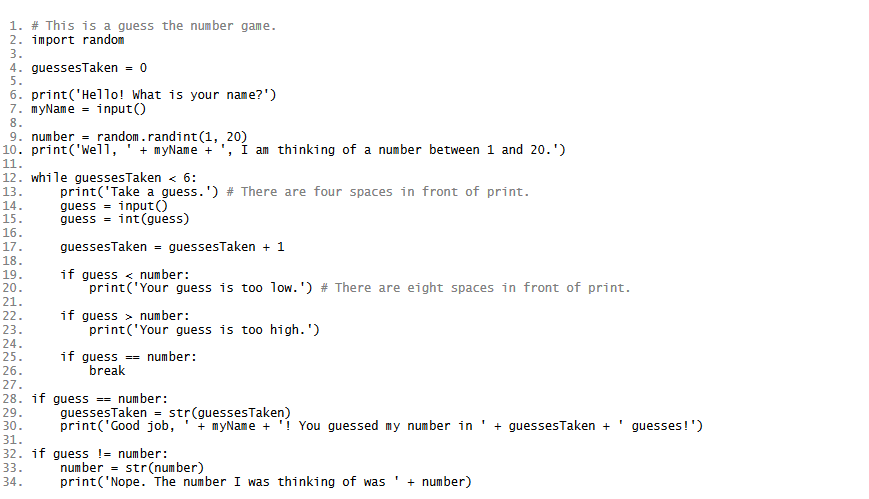
\includegraphics[width=\linewidth,keepaspectratio]{guess}
\end{center}
\end{frame}
